\documentclass[aspectratio=169, compress]{beamer}
% \usetheme{Boadilla}
% \usecolortheme{beaver}

\usetheme{Boadilla}
\usecolortheme{default}
\usepackage{beamerthemesplit}

\usefonttheme{serif}

\usepackage{lipsum}
\usepackage{graphicx,xcolor}
\usepackage{amsmath,amssymb,amsfonts}
\usepackage{tcolorbox}
\tcbuselibrary{theorems}

\usepackage[ruled, vlined]{algorithm2e}
\usepackage{listings}

\definecolor{codegreen}{rgb}{0,0.6,0}
\definecolor{codegray}{rgb}{0.5,0.5,0.5}
\definecolor{codepurple}{rgb}{0.58,0,0.82}
\definecolor{backcolour}{rgb}{1,1,1}

\lstdefinestyle{codestyle}{
    backgroundcolor=\color{backcolour},   
    commentstyle=\color{codegreen},
    keywordstyle=\color{magenta},
    numberstyle=\tiny\color{codegray},
    stringstyle=\color{codepurple},
    basicstyle=\ttfamily\footnotesize,
    breakatwhitespace=false,         
    breaklines=true,                 
    captionpos=b,                    
    keepspaces=true,                   
    numbersep=5pt,                  
    showspaces=false,                
    showstringspaces=false,
    showtabs=false,                  
    tabsize=4
}


\lstset{style=codestyle}

\newtcbtheorem[number within=section]{theo}{Theorem}%
{colback=green!5,colframe=green!35!black,fonttitle=\bfseries}{th}

\newtcbtheorem[number within=section]{lemm}{Lemma}%
{colback=yellow!30,colframe=red!75!black,fonttitle=\bfseries}{th}

\newtcbtheorem[number within=section]{hypothesis}{Hypothesis}%
{colback=red!5,colframe=red!35!black,fonttitle=\bfseries}{th}

\newtcbtheorem[number within=section]{define}{Definition}%
{colback=blue!5,colframe=blue!35!black,fonttitle=\bfseries}{th}

\newtcbtheorem[number within=section]{Fact}{Fact}%
{colback=red!5,colframe=red!35!black,fonttitle=\bfseries}{th}

\title[Packing Coloring Algorithms\hspace{0.5cm}\insertframenumber/\inserttotalframenumber]{Design and Analysis of Algorithms for Packing Coloring}
\institute{\textsc{Indian Institute of Technology Madras}}
\logo{
\includegraphics[height=0.75cm]{iitm.png}}
\author{\href{https://www.theroyakash.com}{theroyakash} and B.V. Raghavendra Rao}

\date{\today{}}


\begin{document}

\maketitle

\section{Introduction}
\begin{frame}{Introduction}
    \begin{itemize}
        \item Goal of the complexity theory is to understand computational difficulty of engineering problems.
    \end{itemize}
\end{frame}

\begin{frame}{Introduction}
    \begin{itemize}
        \item Goal of the complexity theory is to understand computational difficulty of engineering problems.
        \item So we've developed theory to classify problems according to their worst case behaviour. These classes are \textsc{P}, \textsc{NP} etc.
    \end{itemize}
\end{frame}

\begin{frame}{Introduction}
    \begin{itemize}
        \item Goal of the complexity theory is to understand computational difficulty of engineering problems.
        \item So we've developed theory to classify problems according to their worst case behaviour. These classes are \textsc{P}, \textsc{NP} etc.
        \item \textsc{P} class contains all the computational problems that in the worst case completes in polynomial time with respect to the size of the input.
    \end{itemize}
\end{frame}

\begin{frame}{Introduction}
    \begin{center}
        In our \textsc{CS6122} Course we've already seen that real world instances for few NP-Complete problems performs \textbf{good} in terms of running time.
    \end{center}
\end{frame}

\begin{frame}{Introduction}
    \begin{center}
        Thus we must develop theory that'll classify problems of their computational difficulty \textbf{with respect to real world performance} as well. Thus we develop smooth complexity theory.
    \end{center}
\end{frame}

\begin{frame}{Topics we'll look into}
    In this presentation we'll look into the following
    \begin{itemize}
        \item Basic Definitions and assumptions, $\textsf{Smoothed-P}$ Class.
            \begin{itemize}
                \item 2-step vs 1-step model, why we are using one step models,
                \item Support of the distribution, notion of $N_{x, n}$.
                \item Concept of Family of Distribution
                \item Definition of smoothed polynomial running time \textbf{Definition 2.1},
                \item Definition of $\textsf{Smoothed-P}$
                \item \textbf{Theorem 2.3} \textit{An algorithm A has smoothed polynomial running time if and only if there is an} $\epsilon > 0$ \textit{and a polynomial} $p$ \textit{such that for all n, x, $\phi$ and t} $$\Pr_{y \sim D_{n, \phi, x}}[t_A(y; n, \phi) \geq t] \leq \frac{p(n)}{t^\epsilon} N_{n, x} \phi$$
            \end{itemize}
    \end{itemize}

\end{frame}

\begin{frame}{Topics - Continued}
    \begin{itemize}
        \item Heurisitic Schemes, error less heuristic schemes in $\textsf{Smoothed-P}$.
        \item Notion of Reduciblity, define $L_{ds}$, notion of completeness.
            \begin{itemize}
                \item Distributional problems
                \item Polynomial time smoothed reductions $\leq_{smoothed}$
                \item Transitivity of $\leq_{smoothed}$ [via theorem 3.4]
                \item Theorem 3.5 $(L, D) \in \textsf{Smoothed-P}$ if and only if $(L_{ds}, D) \in \textsf{Smoothed-P}^{\textsf{obl}} _{ds}$
            \end{itemize}
    \end{itemize}
\end{frame}


\begin{frame}{Topics - Continued}
    \begin{itemize}
        \item Parameterized Distributional NP $\textsf{Dist-NP}_{\text{para}}$
            \begin{itemize}
                \item Introduction
                \item One $\textsf{Dist-NP}_{\text{para}}$ complete problem to show $\textsf{Dist-NP}_{\text{para}}$ has complete problems
                \item \textbf{Weird looking theorem} \textit{$(\textsf{Tiling}, U^{\textsf{Tiling}})$ is $\textsf{Dist-NP}_{\text{para}}$-complete for some $U^{\textsf{Tiling}} \in \textsf{PComp}_{para}$ under polynomial time smoothed reductions}.
            \end{itemize}

        \item Basic Relation to Worst case complexity
        \item Notion of unsatisfiability and $\textsf{Smoothed-RP}$
        \item Theorem $k \textsf{UNSAT}_{\beta} \in \textsf{Smoothed-RP}$ for $\beta = \Omega(\sqrt{n \log \log n})$
        \item Concluding remarks
    \end{itemize}
\end{frame}

\section{Theory}
\begin{frame}
    \frametitle{Simple Greedy Heuristic for Packing Coloring}

    \begin{itemize}
        \item \textit{We'll start our algorithm to work specifically on trees first because it is easier to analyze and then we'll extend it to general graphs.} \pause[]
        \item \textit{In trees every odd layer we can color with a single color $1$ as every odd layer nodes are at distance more than $1$.}\pause[]
        \item \textit{Hence number of Node remains to be colored is significantly less than the total nodes ($n$). For example a complete $3$-ary tree we can color $75\%$ of the nodes with color $1$.}\pause[]
        \item \textit{We first see how algorithm working on a complete trees. Then we'll look into some of the optimizations we can do to improve the performance of the algorithm.}
    \end{itemize}

\end{frame}

\begin{frame}
    \frametitle{Simple Greedy Heuristic for Packing Coloring}

    \begin{algorithm}[H]\label{alg:1}
        \SetKwInOut{Input}{Input}
    
        \Input{Tree $T$}
        \BlankLine
        Compute Level order traversal of Tree $T$\;
        Color Every Odd layer nodes with \textbf{COLOR(1)}\;
        \texttt{level} $\gets d - 1$ ($d$ is the last level)\;
        \While{\texttt{level} $\geq 0$}{
            \texttt{maximum\_permissible\_color} = $n$\;
            \texttt{current\_color} = $2$\;
            \ForEach{\textsf{Node} in this \textsf{level}}{
                \While{\texttt{current\_color} $<$ \texttt{maximum\_permissible\_color}}{
                    Travel to every node within distance \texttt{( int ) current\_color} and check if there is any node
                    colored with color \texttt{current\_color}\;
                }
            }
        }
        \caption{\textsc{Basic Greedy Algorithm For Any tree}}
    \end{algorithm}

\end{frame}


\begin{frame}
    \frametitle{Simple Greedy Heuristic for Packing Coloring}

    \begin{algorithm}[H]
        \SetKwInOut{Input}{Input}
    
            Travel to every node within distance \texttt{( int ) current\_color} and check if there is any node
            colored with color \texttt{current\_color}\;

            \uIf{None of the node is colored with color \texttt{current\_color}} {
                Color this node with color \texttt{current\_color}\;
                \textbf{break from the loop, go to next node in level}\;
            }\Else{
                \texttt{current\_color} $\gets$ \texttt{current\_color} $+1$\;
            }
            \textsf{level} $\gets$ \textsf{level} $-1$\;
    
        \textbf{Output:} Output this coloring assignment.
    
        \caption{\textsc{Basic Greedy Algorithm For Any tree}}
    \end{algorithm}

\end{frame}

\begin{frame}
    \frametitle{Analysis of the Basic Algorithm}

    \textit{During the analysis we find that there are optimizations we can do to improve the run-time of our algorithm.}

\end{frame}


\begin{frame}
    \frametitle{Complexity Analysis}

    Our algorithm for each node $i \in (1, n)$ in the worst case visits all the $n$ node to find a color (from $1 \to n$). Hence worst case time complexity is $O(n^3)$.

\end{frame}

\begin{frame}
    \frametitle{Optimizations 1}

    We observe one simple fact, that for any complete tree, the maximum number of nodes at any level is present at the last level ($=x^d$, $x$ is the number of children and $d$ is the depth of the last level starting root from $0$).    

\end{frame}


\begin{frame}
    \frametitle{Optimizations 1}

    We are coloring every odd layer with color $1$. \pause[] 
    
    Instead of that if we color the last level and then every alternate level with color $1$ we'll color much more nodes with color $1$ and reduce the total number of colors used. Here is a simple example how this optimization saved thousands of colors.

\end{frame}

\begin{frame}
    \frametitle{Optimizations 1}

    \begin{table}[h]
        \centering
    \begin{tabular}{|l|l|r|l|}
    \hline
    \multicolumn{1}{|l|}{Nodes} & \multicolumn{1}{l|}{Layers} & \multicolumn{1}{l|}{Maximum Colors used} & \multicolumn{1}{l|}{Runtime} \\ \hline
    265720 & 12 & 20633 & 52m 32s 280ms \\ \hline
    265720 & 12 & 6890 & 4m 17s 31ms \\ \hline
    \end{tabular}
    \end{table}

    \pause
    \textit{This one simple optimization reduces the runtime by $92\%$}

\end{frame}



\begin{frame}
    \frametitle{Optimizations 2}

    Suppose we are at the moment trying to color node $u$. Our algorithm for each color $i \in (1, n)$ goes to distance $i$ from the node $u$ and checks if that color exists already or not in all the nodes sitting within distance $i$ from node $u$?

    \pause[]

    \textit{Lets see this step of the basic algorithm with an example.}

\end{frame}

\begin{frame}
    \frametitle{Optimizations 2}

    
    \begin{itemize}
        \item Suppose we are currently looking to color some node $u$ with color $d$.\pause[]
        \item We went to $d$ distance from node $u$ to find all the colors we find. Suppose we find color $d, d + 1, \dots, d+k$ are present in some of the nodes.\pause[]
        \item So we should not check this again for node $u$ with color $d + (1 \to k)$.\pause[]
        \item Hence we implement this modification to improve the runtime.
    \end{itemize}
\end{frame}


\begin{frame}
    \frametitle{Optimizations 2}
    \textit{We define a subroutine called \texttt{Check(u, d)}. This subroutine returns a set of colors present within distance $d$ for any node $u$.}
    \pause[]
    \begin{algorithm}[H]\label{alg:11}
        $\mathcal{C} \gets \phi$\;
    
        Visit all nodes within distance $d$ from node $u$ and collect all the colors into $\mathcal{C}$\;
    
        \textbf{return} Set $\mathcal{C}$\;
        
        \caption{\texttt{Check(Node u, Color d)}}
    \end{algorithm}


    \pause[]
    We can call this subroutine from the main coloring BFS call (we are coloring left to right, level by level). We start with the color $2$ and then we follow the following coloring strategy.
\end{frame}

\begin{frame}
    \frametitle{New coloring strategy}

    \begin{algorithm}[H]
        \For{Each node from last uncolored level, left to right} {
            $d_{\text{prev}}$ $\gets \phi$\;
            \For{Each Color $i$ from $2 \to n$} {
    
                \uIf{Color $i \in d_{\text{prev}}$}{
                It is not possible to color this node with color $i$ because we found color $i$ at distance less than $i$ in $d_{\text{prev}}$\;
                    Continue with color $i + 1$\;
                }
    
                \Else {
                    
                }
            }
        }
        \caption{\texttt{Updated Main Coloring Scheme}}
    \end{algorithm}

\end{frame}


\begin{frame}
    \frametitle{New coloring strategy}

    \begin{algorithm}[H]
        \For{Each node from last uncolored level, left to right} {
            $d_{\text{prev}}$ $\gets \phi$\;
            \For{Each Color $i$ from $2 \to n$} {
                \uIf{Color $i \in d_{\text{prev}}$}{

                }
                \Else{
                    $d_{\text{new}} = $ \texttt{Check(node, i, $d_{\text{prev}}$)}\;
    
                    \uIf{$i \notin d_{\text{new}}$}{
                        Color this node with color $i$\;
                        Break from this loop and start coloring next uncolored node\;
                    } \Else{
                        $d_{\text{prev}} = d_{\text{new}}$
                    }
                }
            }
        }
        \caption{\texttt{Updated Main Coloring Scheme}}
    \end{algorithm}
    
\end{frame}


\begin{frame}
    \frametitle{Optimization 3}

    
    \begin{itemize}
        \item This optimization comes from the observations of the structure of the complete trees.\pause
        \item Complete $x$-ary trees has a depth of $\log_{x} n$ with $n$ many nodes in them.\pause[]
        \item With the following optimization our algorithm time complexity will reduce from $O(n^3)$ down to $O(n d^2)$ for $x$-ary trees with $d$ depth. This is a significant complexity improvement.
    \end{itemize}

\end{frame}

\begin{frame}
    \frametitle{Optimization 3}
    \begin{itemize}
        \item Suppose $j$ is a color that has been used in the tree for the first time (during our run of the algorithm).\pause[] 
        \item If $j >$ the longest path in the tree, then color $j$ can never be used again.\pause[]
        \item Any color after $j$ that is $j + 1$ and so on will also not be possible to reuse.\pause[]
        \item So there is a upper bound on the number of color that are reusable. This depends on the longest path on the tree.
    \end{itemize}    

\end{frame}


\begin{frame}
    \frametitle{Optimization 3}


    \begin{itemize}
        \item For a complete tree longest path is the diameter of the tree. This is equal to $O(\log_{x} n)$ for an complete $x$-ary tree.\pause[]
        \item So in our coloring algorithm we do a simple modification.\pause[]
        \item For each of the node we only check for colors from $1 \to 2*d+2$. The value $2d+2$ is always the upper bound on the color that can be reusable.\pause[]
        \item It is loose bound, can be improved to $\epsilon_1*d \pm \epsilon$ for some fraction $\epsilon_1$ and some integer $\epsilon$. But that would not improve the time complexity of our algorithm.
    \end{itemize}
\end{frame}

\begin{frame}
    \frametitle{Experimental Results}

    We will quickly look at some experimental results on the number of reusable colors and the diameter of the tree.

\end{frame}


\begin{frame}
    \frametitle{Experimental Results}

    \begin{table}[h]
        \centering
        \begin{tabular}{|l|l|}
            \hline
            \textbf{Color number} & \textbf{Number of nodes} \\ \hline
            1                      & 7381                      \\ \hline
            2, 3                      & 738                       \\ \hline
            4, 5                      & 244                       \\ \hline
            6, 7                      & 81                        \\ \hline
            8, 9                      & 27                        \\ \hline
            10, 11                     & 9                         \\ \hline
            12, 13                     & 3                         \\ \hline
            14 $\to$ 269  & 1\\ \hline
        \end{tabular}
        \caption{Number of nodes colored with each color for a 9-layer complete tree.}
        \label{tab:colors}
    \end{table}

\end{frame}

\begin{frame}
    \frametitle{Mathematical Analysis}

    
    \begin{itemize}
        \item We look into some of the properties of the algorithm, how it performs on a three-ary complete tree.\pause[]
        \item We'll analyse a upper-bound on the number of colors used in the graph, and a bound on the number of nodes are colored by certain color.
    \end{itemize} 
\end{frame}

\begin{frame}
    \frametitle{Total color upper bound}

    We need to prove a upper bound on the number of colors used by our algorithm.    

\end{frame}

\begin{frame}
    \frametitle{Total color upper bound}

    To prove this if we could prove how many nodes are colored by each of the colors (or their upper bound) then we can count the total number of colors used by the algorithm.    

\end{frame}


\begin{frame}
    \frametitle{Theoretical Bounds}

    \textit{First we analyze the number of nodes colored with color $1$.}
\end{frame}

\begin{frame}
    \frametitle{Number of Nodes with Color 1}

    \begin{align*}
        \frac{\textsf{Total Color 1 Nodes}}{\textsf{Total Nodes}} &= \frac{3^{x} + 3^{x - 2} + 3^{x-4} + \dots 3^{1}}{\displaystyle\sum_{i = 0} ^{i = x} 3^i}\\
    \end{align*}

    \textit{If number of layers is odd ($x$ is odd) then the upper part of the fraction stops at $1$ and $0$ otherwise.}

\end{frame}

\begin{frame}
    \frametitle{Number of Nodes with Color 1}

    \begin{align*}
        \textsf{Ratio of Color 1 node to total nodes} &= \frac{3^{x} + 3^{x - 2} + 3^{x-4} + \dots 3^{1}}{\displaystyle\sum_{i = 0} ^{i = x} 3^i}\\
        &= \frac{3 \cdot \frac{9^{\frac{x}{2}} - 1}{9 - 1}}{\frac{3^x - 1}{2}}\\
        &= \frac{3}{4} \cdot \frac{3^x - 1}{3^x - 1}\\
        &= \frac{3}{4}
    \end{align*}    

\end{frame}

\begin{frame}
    \frametitle{Number of Nodes with Color 1}

    \begin{Fact}{Total Nodes with color 1}{}
        For complete trees we can color at most $\frac{3}{4}$ many nodes with color 1.
    \end{Fact}

\end{frame}

\begin{frame}
    \frametitle{Number of Nodes with Color 2}

    To count how many nodes are colored with color $2$ we'll approach this problem inductively.    

\end{frame}

\begin{frame}
    \frametitle{Number of nodes with color 2}


    \begin{itemize}
        \item First we find out for small size trees (for example level $3$ trees) how many nodes are colored with color $2$.\pause[]
        \item Then we extrapolate this to bigger trees. This analysis holds because bigger complete tree has these smaller complete threes as their children.
    \end{itemize}

\end{frame}

\begin{frame}
    \frametitle{Number of nodes with color 2}

    \begin{figure}
        \centering
        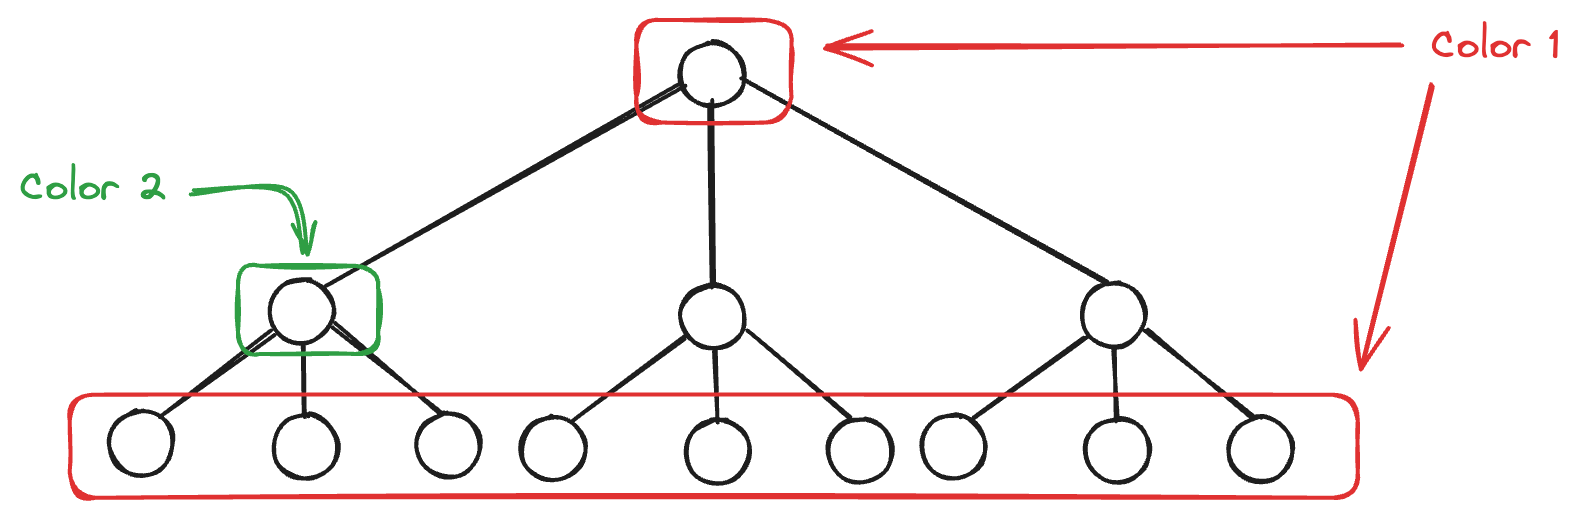
\includegraphics[width=0.7\linewidth]{images/layer 3.png}
        \caption{For a three layer deep tree only one node can be colored with Color $2$}
        \label{fig:enter-label}
    \end{figure}

\end{frame}

\begin{frame}
    \frametitle{Number of nodes with color 2}

    So for a four layer tree, the total number of nodes colored with color $2$ is $3 \times 1 = 3$

\end{frame}


\begin{frame}
    \frametitle{Number of nodes with color 2}

    \begin{itemize}
        \item Layer $4$ tree is a combination of $3$ layer $3$ trees connected with one extra node.\pause[]
        \item This extra node can not be colored with color $2$. Hence total color $2$ needed is three times the total color $2$ in the $3$ layered tree.    
    \end{itemize}

\end{frame}

\begin{frame}

    \frametitle{Number of nodes with color 2}
    
    
    \begin{itemize}
        \item Same thing is true for layer $5$ tree also because the extra node (top most node) here will be colored with color $1$ as odd layers are colored with color $1$.\pause[]
        \item At layer $6$ the top most node can be colored with color $2$. Hence for layer six the number of node is one more of $3$ times the number of nodes colored in layer $5$ tree.\pause[]
        \item We see a deviation from this pattern in layer $7$ tree.
    \end{itemize}

\end{frame}

\begin{frame}
    \frametitle{Layer 6 Trees}

    
    \begin{itemize}
        \item In layer $6$ tree we have $3$ layer $5$ trees connected with one extra node. The top most node is colored with color $2$\pause[]
        \item Each of the layer $6$ tree has $28$ nodes colored with color $2$.\pause[]
        \item However we can not combine these three layer $6$ trees with one extra node. Because the top most node in the layer $6$ colored with color $2$ will violate the distance conditions in the layer $7$ tree.\pause[]
        \item So we can only have one of the children (layer $6$) with color $2$ and rest are not colored with color $2$.\pause[]
        \item Hence we need to subtract $2$ from three times the total number of nodes colored with color $2$ in layer $6$ tree to count color $2$ nodes in layer $7$ trees.
    \end{itemize}

\end{frame}

\begin{frame}
    \frametitle{Generalization}

    Extending this concept to larger and larger trees we can see a pattern.
    
    \pause[]

    \begin{align*}
        A &= [0, 0, 1, -2]\\
        f_2(x) &= A[x \% 4] + 3 \cdot f_2(x - 1)
    \end{align*}


    \pause[]

    We use $f_2(3) = 1$ as the base-case. 

\end{frame}

\begin{frame}
    \frametitle{Approximation of number of nodes colored with color $2$}

    \begin{lemm}{Color $2$ node count}{}
        Simple greedy heuristic for complete tree packing coloring, colors roughly $\frac{1}{10} ^{\text{th}}$ many nodes with color $2$ as compared to color $1$.
    \end{lemm}

\end{frame}

\begin{frame}
    \frametitle{Proof}

    \begin{hypothesis}{}{}
        Suppose $f_2(x - 1) \approx \frac{1}{10} \cdot \frac{3}{4} \cdot \displaystyle\sum_{i = 0} ^{x - 2} 3^i$ is the number of color $2$ used by our algorithm for a $x - 1$ layer deep tree. 
    \end{hypothesis}

    We need to prove $f_2(x) \approx \frac{1}{10} \cdot \frac{3}{4} \cdot \displaystyle\sum_{i = 0} ^{x - 1} 3^i$ and verify this with experimental results.
\end{frame}

\begin{frame}
    \frametitle{Proof Continued}

    Using induction hypothesis and previous results we get,
    \begin{align*}
        f_2(x) &= A[x\%4] + 3 \cdot f_2(x - 1)\\
        &= A[x\%4] + 3 \cdot \frac{1}{10} \cdot \frac{3}{4} \cdot \displaystyle\sum_{i = 0} ^{x - 2} 3^i\\
        &= A[x\%4] + \frac{3}{4} \cdot \frac{1}{10} \cdot \displaystyle\sum_{i = 0} ^{x - 1} 3^i\\
        &\approx \frac{1}{10} f_1(x)
    \end{align*}

    Here $A[i] \in \{-2, 0, 1\}$, hence $f_2(x)$ is roughly $\frac{1}{10} \cdot f_1(x)$ where $f_1(x)$ is the number of color $1$ used.    

\end{frame}

\begin{frame}
    \frametitle{Results for other colors}

    We can also use these similar arguments for other higher colors, with that we can say the following facts\pause[]
    
    \begin{itemize}
        \item For three-ary complete trees number of nodes colored with color $(2, 3), (4, 5), (6, 7), \dots$ are the same pairwise,\pause[]
        \item For three-ary complete trees number of nodes colored with color $(4, 5),$ is one-third of the number of nodes colored with $(2, 3)$ and so on,\pause[]
        \item After a while when some pair of colors $(x, x + 1)$ are used $\leq 3$ times, all the colors from $x + 2$ and so on are used only once.
    \end{itemize}

\end{frame}

\begin{frame}
    \frametitle{Total Color upper bound}

    Now we prove the upper bound on the number of colors used by our algorithm.    

\end{frame}

\begin{frame}
    \frametitle{Total color upper bound}

    \begin{theo}{$n/40$ scheme}{}
        \textit{Simple greedy heuristic is a $\frac{n}{40}$ approximation algorithm for complete three-ary trees.}
    \end{theo}

\end{frame}

\begin{frame}
    \frametitle{Proof}

    Say we are coloring an $x$ layer deep complete three ary tree with total number of node $= n$ and 
    
    \[n = \displaystyle\sum_{i = 0} ^{x - 1} 3^i\]

\end{frame}

\begin{frame}
    \frametitle{Proof contd.}

    \begin{itemize}
        \item Number of nodes colored with color $1 = \frac{3n}{4}$
        \item Number of nodes colored with color $2, 3 = \frac{3n}{40}$
        \item Number of nodes colored with color $4, 5 = \frac{n}{40}$
        \item Number of nodes colored with color $6, 7 = \frac{n}{120}$
        \item Number of nodes colored with color $8, 9 = \frac{n}{360}$
        \item \dots
    \end{itemize}    

\end{frame}

\begin{frame}
    \frametitle{Proof Contd.}

    We say $j = 1$ at color $2, 3$, from there on $j$ stops at $j = j$ when $\frac{n}{n} = 1$. From there on rest of all the nodes are colored with an non-reusable color.

\end{frame}

\begin{frame}
    \frametitle{Proof Contd.}

    Total number of different colors used $= 1 + 2\cdot j + \textsf{ number of non-reusable colors}$. We now need to calculate the number of non-reusable colors and the value of $j$. Value of $j$ when the denominator becomes $n$ is when re-usable colors are finished.    

\end{frame}

\begin{frame}
    \frametitle{Proof Contd.}

    \begin{align}
        \textsf{Total non-reusable color} &= n - \left[ \frac{3n}{4} + 2 \cdot \left( \frac{3n}{40} + \frac{n}{40} + \frac{n}{40 * 3} + \frac{n}{40 * 3^2} \dots + 1 \right)\right]
    \end{align}

    First we calculate $\left( \frac{3n}{40} + \frac{n}{40} + \frac{n}{40 * 3} + \frac{n}{40 * 3^2} \dots + 1 \right)$.

    \begin{align*}
        s_n &= \left( \frac{3n}{40} + \frac{n}{40} + \frac{n}{40 * 3} + \frac{n}{40 * 3^2} \dots + 1 \right)\\
        &= \frac{3n}{40} \left[ \frac{1 - \left(\frac{1}{3}\right)^{2 + \log_3\left(\frac{n}{40}\right)}}{1 - \frac{1}{3}} \right]\\
        &= \frac{9n}{80} - \frac{1}{2}
    \end{align*}    

\end{frame}

\begin{frame}
    \frametitle{Proof Contd.}

    We put this into the equation (1), then we get
    \begin{align*}
        &= n - \left[\frac{3n}{4} + 2 \cdot \left(\frac{9n}{80} - \frac{1}{2}\right)\right]\\
        &= \frac{n}{40} + 1
    \end{align*}    

\end{frame}

\begin{frame}
    \frametitle{Proof Contd.}

    We put this calculation into the original equation to get the total number of colors used as
    \begin{align}
        \textsf{Total colors used} &= 1 + 2 \cdot \left[\log_3\left(\frac{n}{40} + 2\right)\right] + \frac{n}{40} + 1\\
        &\geq \frac{n}{40}
    \end{align}

\end{frame}

\begin{frame}
    \frametitle{Proof contd.}

    For very large $n$ expression (2) evaluates to almost $\frac{n}{40}$. This proves our lemma saying, our simple greedy algorithm outputs a valid packing coloring assignment with at-least $\frac{n}{40}$ many colors.    

\end{frame}

\section{Expt. Results and Future}
\begin{frame}
    \frametitle{Experimental Results}
    Here I'll show how the experimental results support our theoritical analysis.
\end{frame}

\begin{frame}
    \frametitle{Experimental Results}

    \begin{table}[h]
        \centering
        \begin{tabular}{|l|l|l|l|l|}
        \hline
        \# of Nodes & \# of Layers & X-ary tree & Total Colors & Time\\
        \hline
        13 & 3 & 3 & 4 & 0ms \\\hline
        40 & 4 & 3 & 7 & 0ms \\\hline
        121 & 5 & 3 & 11 & 2ms \\\hline
        364 & 6 & 3 & 19 & 6.11029 ms \\\hline
        1093 & 7 & 3 & 40 & 38ms \\\hline
        3280 & 8 & 3 & 98 & 63ms \\\hline
        9841 & 9 & 3 & 269 & 1s 101ms \\\hline
        29524 & 10 & 3 & 781 & 3s 845ms \\\hline
        88573 & 11 & 3 & 2309 & 45s 256ms \\\hline
        265720 & 12 & 3 & 6890 & 4m 17s 31ms \\ \hline
        7174453 & 15 & 3 & 185525 & 9 days 7 hours 29 min 9 sec\\
        \hline
        \end{tabular}
        \caption{Runtime, total color used for a complete three-ary tree.}
        \end{table}
\end{frame}

\begin{frame}
    \frametitle{Total Colors Used}

    All the experimental results show that the total number of colors used is less than $\frac{n}{40}$ where $n$ is the number of nodes in the tree. 
    
    \pause[]
    This is in line with our theoritical analysis.

\end{frame}

\begin{frame}
    \frametitle{Total Colors Used}

\begin{table}[h]
    \centering
    \begin{tabular}{|l|l|}
        \hline
        \textbf{Color number} & \textbf{Number of nodes} \\ \hline
        1                      & 5380840                   \\ \hline
        2, 3                      & 538084                    \\ \hline
        4                      & 177391                    \\ \hline
        5                      & 177390                    \\ \hline
        6, 7                   & 59058                     \\ \hline
        8, 9                   & 19684                     \\ \hline
        10, 11                 & 6561                      \\ \hline
    \end{tabular}
    \caption{Number of nodes colored with each color for a 15-layer complete tree.}
    \label{tab:colors}
    \end{table}
\end{frame}


\begin{frame}
    \frametitle{Total Colors Used}
    \begin{table}[h]
        \centering
        \begin{tabular}{|l|l|}
            \hline
            \textbf{Color number} & \textbf{Number of nodes} \\ \hline
            12, 13                 & 2187                      \\ \hline
            14, 15                 & 729                       \\ \hline
            16, 17                 & 243                       \\ \hline
            18, 19                 & 81                        \\ \hline
            20, 21                 & 27                        \\ \hline
            22, 23                 & 9                         \\ \hline
            24, 25                 & 3                         \\ \hline
            26 $\to$ 185525  & 1\\ \hline
        \end{tabular}
        \caption{Number of nodes colored with each color for a 15-layer complete tree.}
        \label{tab:colors}
    \end{table}
\end{frame}

\begin{frame}
    \frametitle{Experimental Results}

    These experimental results prove the following things

    \pause[]


    \begin{itemize}
        \item Color $2$ is used $\frac{1}{10}$th of the total number of nodes colored with color $1$.\pause[]
        \item Color $1$ is used for the $\frac{3}{4}^{\text{th}}$ of the total number of nodes.\pause[]
        \item Pair-wise colors are used for the same amount of nodes in the tree.\pause[]
        \item After $26$ which is some less than $2*d = 2*15 = 30$, all the colors are used for only once.
    \end{itemize}

\end{frame}

\begin{frame}
    \frametitle{Conclusion}

    This completes our presentation on the approximation algorithm for packing coloring on trees.

    \pause[]

    \textit{In future we'll look for the following things:}\pause[]
    
    \begin{itemize}
        \item We analysed our algorithm performance on a complete three-ary tree and some trees with randomly delete branch. We need to analyse the performance for any $d$-degree bounded tree and graphs. To do this one approach we thought of is to design an algorithm that'll find a suitable root such that most of the nodes are equidistant from this root. Suitable root must decrease the number of colors to be used by our algorithm.\pause[]
        \item To test the effectiveness of the algorithm we need to come up with a random-graph generation scheme. Through which we can generate graphs at random with certain properties and review our algorithm performance.\pause[]
    \end{itemize}
    
\end{frame}

\begin{frame}
    \frametitle{Future}


    \begin{itemize}
        \item We need to come up with a randomized graph generation scheme that'll generate worst case graphs to color for our algorithm. This will generate the worst case graphs, that'll cost very significant amount of colors to color according to our coloring strategy and some fix for those graphs. We also need to check the performance of our algorithm on randomly chosen graph from a fixed distribution.
    \end{itemize}

\end{frame}

\begin{frame}
    \frametitle{Thank You}

    \begin{center}
        \Huge{Thank You}
    \end{center}

\end{frame}

\end{document}